\documentclass{article}
\usepackage[utf8]{inputenc}
\usepackage[T1]{fontenc} 
\usepackage[slovene]{babel} 

\usepackage{enumitem} 
\usepackage{hyperref}
\usepackage{amsmath}
\usepackage{amsthm} 
\usepackage{amssymb}
\usepackage{lmodern}
\usepackage{amsfonts} 
\usepackage{mathtools}
\usepackage{graphicx}
\usepackage{float}

\DeclareMathOperator{\EX}{\mathbb{E}}
%\setlength{\abovecaptionskip}{15pt plus 3pt minus 2pt}

\begin{document}

\title{Simetrična diskretna verižnica z liho členki\\
    \large Projekt pri predmetu Statistika
}
\author{
    Matej Novoselec\\
}
\date{30.\ junij 2023}

\maketitle

\begin{figure}[H]
    \begin{center}
    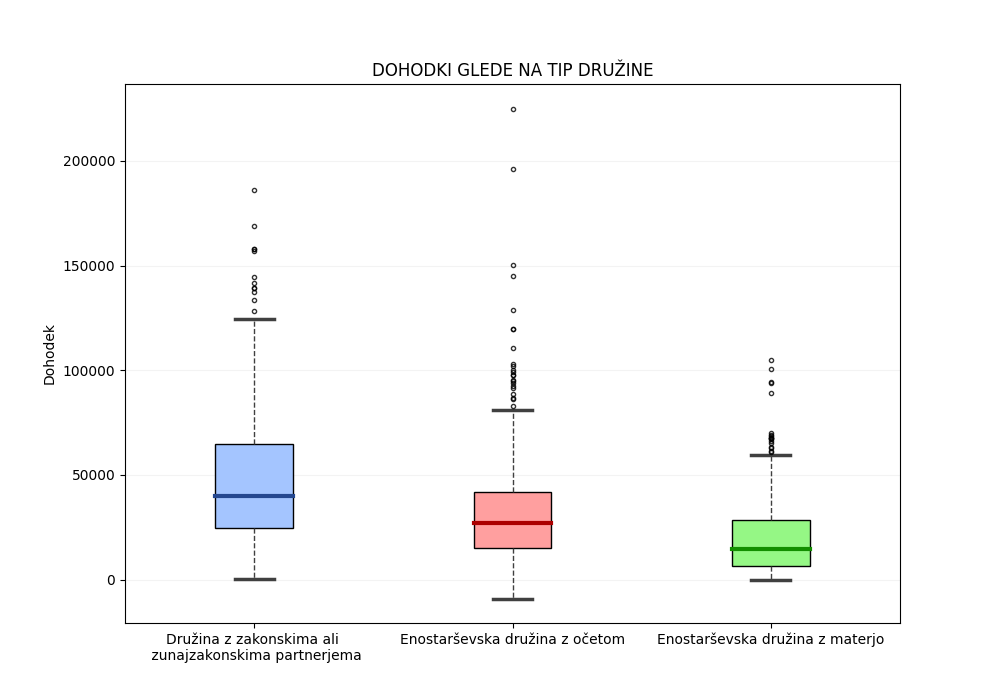
\includegraphics[width=\linewidth]{naloga1a.png}
    \vspace*{-10mm}\caption{Škatle z brki za dohodke različnih tipov družin}
    \end{center}    
\end{figure}


\begin{figure}[H]
    \begin{center}
    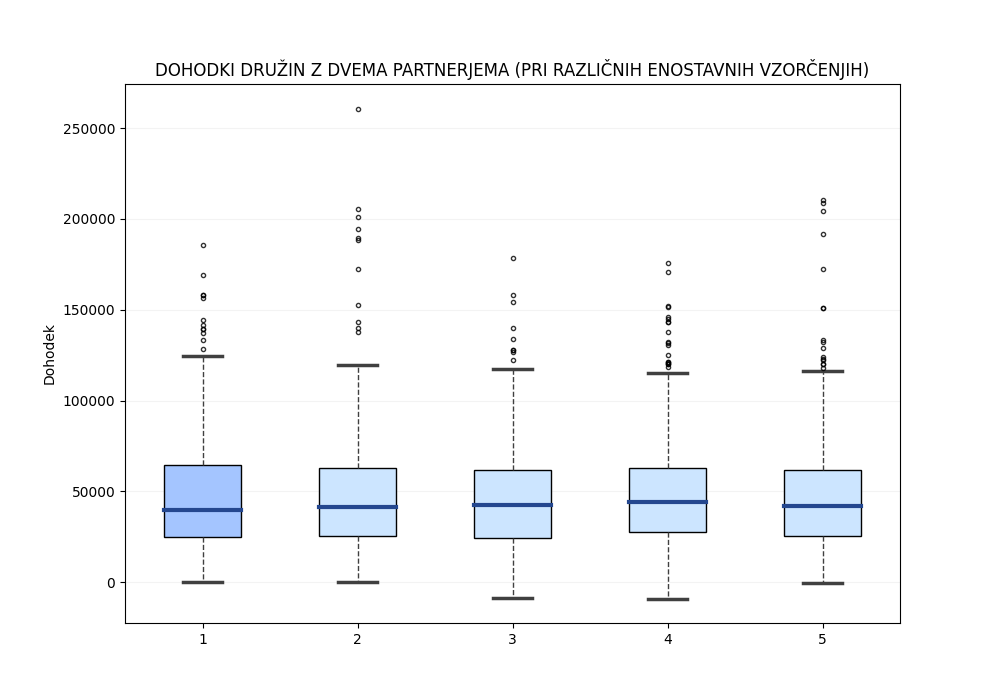
\includegraphics[width=\linewidth]{naloga1b.png}
    \vspace*{-10mm}\caption{Škatle z brki za dohodke družin z dvema partnerjema}
    \end{center}    
\end{figure}


\pagebreak

\section{Naloga 2}
Vredno je zapisati nekoliko bolj matematično interpretacijo problema/navodila. 
Podatki pripadajo trem različnim eksperimentom, ki bodo določali končne vrednosti in rezultate, a so problemi, ki jih podajajo, teoretično iste narave. 
Za podan problem sedaj razvijemo teoretični pristop in se lotimo reševanja podnaloge a) in b). 
\newline
Imamo $n$ neodvisnih, enako porazdeljenih slučajnih spremenljivk, označimo jih z $R_1,~R_2,~\dots,~R_n$. 
Porazdeljene naj bodo Rayleighovo, t.j. z gostoto:
$$
f_{R_i}(r_{i} \mid \theta)=\left\{\begin{array}{cl}
\frac{r_i}{\theta^{2}} \exp \left(-\frac{r_{i}^{2}}{2 \theta^{2}}\right) & ;~~r>0 \\
0 & ;~~\text{sicer }
\end{array}\right. .
$$
Zaradi predpostavljene neodvisnosti, je potem $(R_1,~R_2,~\dots,~R_n)$ porazdeljen z gostoto:
$$
    \prod_{i=1}^{n}{f_{R_i}(r_{i} \mid \theta)} = 
    \bigg(\frac{1}{\theta^{2n}}\prod_{i=1}^{n}{r_i}\bigg) \exp\bigg(-\frac{1}{2 \theta^{2}} \sum_{i=1}^{n}{r_i^2}\bigg);~~r_i>0.
$$
Lotimo se podnaloge a). Velja:
$$
L(\theta \mid (r_1,~r_2,~\dots,~r_n)) = \prod_{i=1}^{n}{L_i(\theta \mid r_i)} = \prod_{i=1}^{n}{f_{R_i}(r_i \mid \theta)}
$$
in
$$
l(\theta \mid (r_1,~r_2,~\dots,~r_n)) = \ln L(\theta \mid (r_1,~r_2,~\dots,~r_n)) = \sum_{i=1}^{n}{\ln \big(f_{R_i}(r_i \mid \theta)\big)}, 
$$
ter zato:
$$
l(\theta \mid (r_1,~r_2,~\dots,~r_n)) = -2n \ln(\theta) + \sum_{i=1}^{n}{\ln(r_i)} - \frac{1}{2\theta^2} \sum_{i=1}^{n}{r_i^2}~.
$$
Iščemo cenilko za $\theta$ po metodi največjega verjetja, zato si ogledamo enakost:
$$
0 = \frac{\partial l(\theta \mid (r_1,~\dots,~r_n))}{\partial \theta} = - \frac{2n}{\theta} + \frac{1}{\theta^3}\sum_{i=1}^{n}{r_i^2}.
$$
Za cenilko po metodi največjega verjetja tako dobimo:
$$
\hat{\theta}_{MNV} = \sqrt{\frac{1}{2n}{\sum_{i=1}^{n}{r_i^2}}}~.
$$
Za rešitev podnaloge b) si oglejmo pričakovano vrednost (Rayleighove) slučajne spremenljivke $R$:
$$
\EX(R) = \int_{0}^{\infty}{r~f(r \mid \theta)~dr}= \int_{0}^{\infty}{\frac{r^2}{\theta^{2}}~\exp\Big(-\frac{r^{2}}{2 \theta^{2}}\Big)~dr}.
$$
Uvedemo $\tau = \frac{r^{2}}{2 \theta^{2}}$ in dobimo
$$
\EX(R) = \int_{0}^{\infty}{\sqrt{2 \tau}~\theta ~e^{-\tau}~ d \tau} = \theta \sqrt{2}\int_{0}^{\infty}{\tau^{1/2}~e^{-\tau}~ d \tau} = \theta\sqrt{2}~\Gamma(3/2) = \theta \sqrt{\frac{\pi}{2}}.
$$
Cenilka po metodi momentov je zato podano s predpisom:
$$
\hat{\theta}_{MM} = \overline{R} \sqrt{\frac{2}{\pi}}.
$$
Iz izpeljave cenilke, dobljene po metodi momentov, je jasno vidno, da je cenilka nepristranska (hitro bi lahko tudi direktno preverili, da res velja $\EX(\hat{\theta}_{MM}) = \theta$).
\newline
Na podoben način, kot smo to storili zgoraj, se dokopljemo do pomožnega rezultata, ki nam bo prav prišel kasneje. Velja:
$$
\EX(R^2) = \int_{0}^{\infty}{r^2~f(r \mid \theta)~dr}= 2 \theta^2.
$$
\newline
\newline
Sedaj se lotimo reševanja podnaloge c). Ker je cenilka za $\theta$ po metodi momentov nepristranska, velja $MSE(\hat{\theta}_{MM}) = Var(\hat{\theta}_{MM})$. Sedaj varianco tudi poračunajmo.
\begin{equation*}
    \begin{split}
    Var(\hat{\theta}_{MM}) = Var\bigg(\overline{R} \sqrt{\frac{2}{\pi}}\bigg) = \frac{2}{\pi} \frac{Var(R)}{n} = \frac{2}{\pi}\frac{\EX(R^2) - (\EX(R))^2}{n} = \\
    = \frac{2}{\pi}\bigg(\frac{2 \theta^2 - \big(\frac{\pi}{2} \theta\big)^2}{n}\bigg) = \frac{\theta^2}{n} \bigg(\frac{4 - \pi}{\pi}\bigg)
    \end{split}
\end{equation*}
Po zgornjem komentarju torej
$$
MSE(\hat{\theta}_{MM}) = \frac{\theta^2}{n} \bigg(\frac{4 - \pi}{\pi}\bigg)\approx \frac{\theta^2}{n} \cdot 0{,}273.
$$
Pri izračunu asimptotične srednje kvadratične napake pri cenilki za $\theta$ po metodi največjega verjetja, nam na pomoč priskoči Fischerjeva informacija. 
Velja:
\begin{equation*}
    \begin{split}
    FI(\theta) = - \EX\bigg(\frac{\partial^2 l(\theta \mid (r_1,~\dots,~r_n))}{\partial \theta^2}\bigg) = -\EX\bigg(\frac{1}{\theta^4}\bigg(2n\theta^2 - 3 \sum_{i=1}^{n}{r_i^2}\bigg)\bigg) = \\
    = -\EX\bigg(\frac{1}{\theta^4}\bigg(2n \theta^2 - n \EX(R^2)\bigg)\bigg) = -\EX\bigg(\frac{1}{\theta^4}\bigg(2n \theta^2 - 3n \Big(\frac{\pi}{2} \theta^2 + \frac{4- \pi}{2}\theta^2\Big)\bigg)\bigg) = \frac{4n}{\theta^2}, 
    \end{split}
\end{equation*}
oziroma: 
$$ 
    FI^{-1}(\theta) = \frac{1}{4}\frac{\theta^2}{n},~\text{zato asimptotično velja:}~~MSE(\hat{\theta}_{MNV}) \approx \frac{\theta^2}{n} \cdot 0{,}25. 
$$
Opazimo, da je faktor pred asimptotično srednje kvadratično napako za cenilko, dobljeno po metodi največjega verjetja nekoliko manjši, zato je vsaj asimptotično cenilka $\hat{\theta}_{MNV}$ nekoliko boljša od cenilke $\hat{\theta}_{MM}$.



\bibliographystyle{siam}
\begin{thebibliography}{9}
    \bibitem{clanek}
        E.~Zakrajšek, \emph{Verižnica}, [ogled 30.~6.~2023], dostopno na \url{https://ucilnica.fmf.uni-lj.si/pluginfile.php/8283/mod_resource/conte4/predavanja/veriznica/veriznica.pdf}.
    \bibitem{zapiski}
        E. Žagar \emph{Zapiski predavanj 22.3.2021 - Problem diskretne verižnice} [ogled 29.~6.~2023], dostopno na \url{https://ucilnica.fmf.uni-lj.si/pluginfile.php/100122/mod_resource/content/1/mm_uni_22_3_21.pdf}.
\end{thebibliography}

\end{document}